\begin{savequote}[10cm] % this sets the width of the quote
\sffamily
I'm sure there are some things out there that OpenDoc does..that I'm not familiar with that nothing else out there does\ldots and I'm sure you can make some demos, maybe a small commercial app, that demonstrates those things.
\ldots
One of the things I've always found is that you've gotta start with the customer experience and work backwards to the technology.
\ldots
It started with 'what incredible benefits can we give to the customer; where can we take the customer' not 'let's sit down with the engineers, figure out what awesome technology we have and then how are we going to market that' \ldots And I think that's the right path to take.
\qauthor{Steve Jobs -- Apple World Wide Developer Conference Keynote, 1997}
\end{savequote}

\chapter{Technology} 

\section{Main Message}
The technology to allow access to the internet is improving but other countries have more universal access to the internet than the majority of people in Australia. People in regional and remote areas have disproportionately more issues connecting to the internet than people in urban areas.

Australia has historically been a heavy user of communications technology. Indigenous people passed messages between populations by physical movement and spoken language. At different times of the year or during different seasons they would migrate to obtain a better living and would exchange stories and information with other Indigenous people on the way as they passed through their nations\cite{RefWorks:453}. Non-Indigenous people employed physical mail delivery and eventually moved to electronic communications such as telegraph, telephone and satellite. Satellite communications have been emphasised as a solution to remote and very remote communications users but they are only part of the solution. The current technology mix in Australia favours life extension of the existing copper network, mobile and static telephone communications technologies such as \Gls{lte} and commercial mobile data technologies. Access to Technology and to the internet is a precondition to deriving benefit from the internet but full utility is not realised until several other preconditions are satisfied. Future technologies may address the shortcomings of the existing network and the availability and adoption curve of these technologies can be simulated using previous experience in markets that adopt technology at a similar rate to Australia. 



\section{Mobile Broadband in Australia}

It is often assumed that remoteness makes internet access difficult, that if the network is brought to the user then that user will be able to use the internet. Mobile phone and NBN coverage maps show large geographical areas of Australia are covered and that these coverage areas provide at least basic service to the majority of the population. Access to the internet is required but is not sufficient for people to use the internet. Telstra's research on the barriers to access for remote and very remote internet users found that it wasn't only the provision of network service that prevented their customers using the internet in remote and very remote Australia. In the \textit{Connect, Innovate and Support}\cite{RefWorks:230} survey, they found that the ability to access a network service at high service quality and speed was not sufficient to enable or in some cases, motivate, potential users to take advantage of the benefits the internet had to offer them. They found the barriers to use were:

\begin{enumerate}
\item{Infrastructure:} this barrier is essentially about the `pipes' to
the home, community or organisation office.
\item{Hardware in the home:} this goes to the logistics and support
that is necessary to get modems, computers or wifi into the
home or in the provision of community services such as
community wifi or hubs.
\item{Affordability:} this barrier is about people's ability and willingness
to pay for data and other digital services and devices.
\item{Propensity:} this barrier is about the ability and desire of individuals
to take up and use digital services and technology.
\item{Appropriate web based services:} this is about the barrier
created when websites are very wordy and difficult to navigate\cite{RefWorks:230}.
\end{enumerate}

\begin{figure}[ht]
\centering
\includegraphics[scale=.5]{figures/Barriers-to-use.png}
\caption{Barriers to use of internet in non-urban areas \cite{RefWorks:230}}
\label{fig:barrierstouse}
\end{figure}
They went further to quantify the degree to which each of these barriers was a burden on the customer and the order in which they should be satisfied (Figure \ref{fig:barrierstouse}).


\subsection{The Mobile Broadband Network}





Figure~\ref{fig:ConnectionType} shows that the majority of the respondents used a wired connection to respond. The ABS's most recent survey on internet use showed that 91.4\% of households used a desktop computer but also that 91\% of households used mobile or smartphone technology to access the internet\cite{RefWorks:459}. 

Respondents with wired connections used NBN, Optus or Telstra cable internet (26 respondents), NBN fibre (8 respondents) with the majority using ADSL (56 respondents) and ADSL2+ (95 respondents). Only three respondents still admitted to using dial-up internet, two of which were in Major Cities of Australia and the other was in Outer Regional Australia so remoteness did not seem to indicate automatic selection of inferior access methods. Of the 66 respondents that used the highest speed access methods of cable and NBN, 45 or 13\% of all respondents, were in non-MCA areas.

\begin{figure}
\centering
\wheelchart{16/mqDarkRed/Mobile,  84/mqGreyRed/Wired}
\caption{Connection Type}
\label{fig:ConnectionType}
\end{figure}

105 respondents used `wireless' technology for their internet access. At 82 respondents, WiFi was the most popular wireless technology which either indicated that the person was actually using a mobile broadband hotspot or cable through a wireless router or it may have indicated that the person's primary internet connection was through public or work provided WiFi hotspots. 23 respondents used 4G mobile broadband and only 10 used 3G broadband. 13 respondents were unsure how they were getting their internet.

\begin{figure}
\centering
\wheelchart{40/mqDarkRed/Cable,  10/mqGreyRed/Fibre, 49/mqRed/Wired, 33/mqPlum/Wireless}\label{fig:ConnectionTech}
\caption{Connection Technology}
\end{figure}

The trend in internet connections in developing markets is for a `Negroponte Switch', named after Nicholas Negroponte's observation that those communications technologies that had be wireless would increasingly use wireless technology and wireless communications technologies would become wired.\cite{RefWorks:361} While this survey showed most people used wired technologies to access the internet, it may be that, with the increasing prevalence of mobile devices being used on a regular basis, PCs connected to wired connections will be less popular in the future.



\begin{figure}
\centering
\wheelchart{40/mqDarkRed/Dial-up to 1Mbps,  28/mqGreyRed/2-8Mbps,  34/mqRed/{8-40Mbps}, 15/mqPlum/{\textgreater 40Mbps}, 228/mqLightPlum/{Not Sure}}
\caption{Connection Speeds}
\label{fig:ConnectionSpeed}
\end{figure}

Although much attention is paid to the speed of internet downloads in complaints to the NBN and in anecdotal comments generally, most of the respondents to this survey indicated that they didn't know how fast their internet connection was. Less than five percent knew that they had a broadband speed of over 40Mbps and fewer than ten percent (34 respondents) reported a speed that was above ADSL speed. 

%need to do sentiment analysis of people's impressions of their service here.

\subsection{How Australians access the internet in different regions}

\begin{figure}
\centering
%\includepdf[pages={1}, angle=270, scale=0.5]{figures/myplot-1.eps}
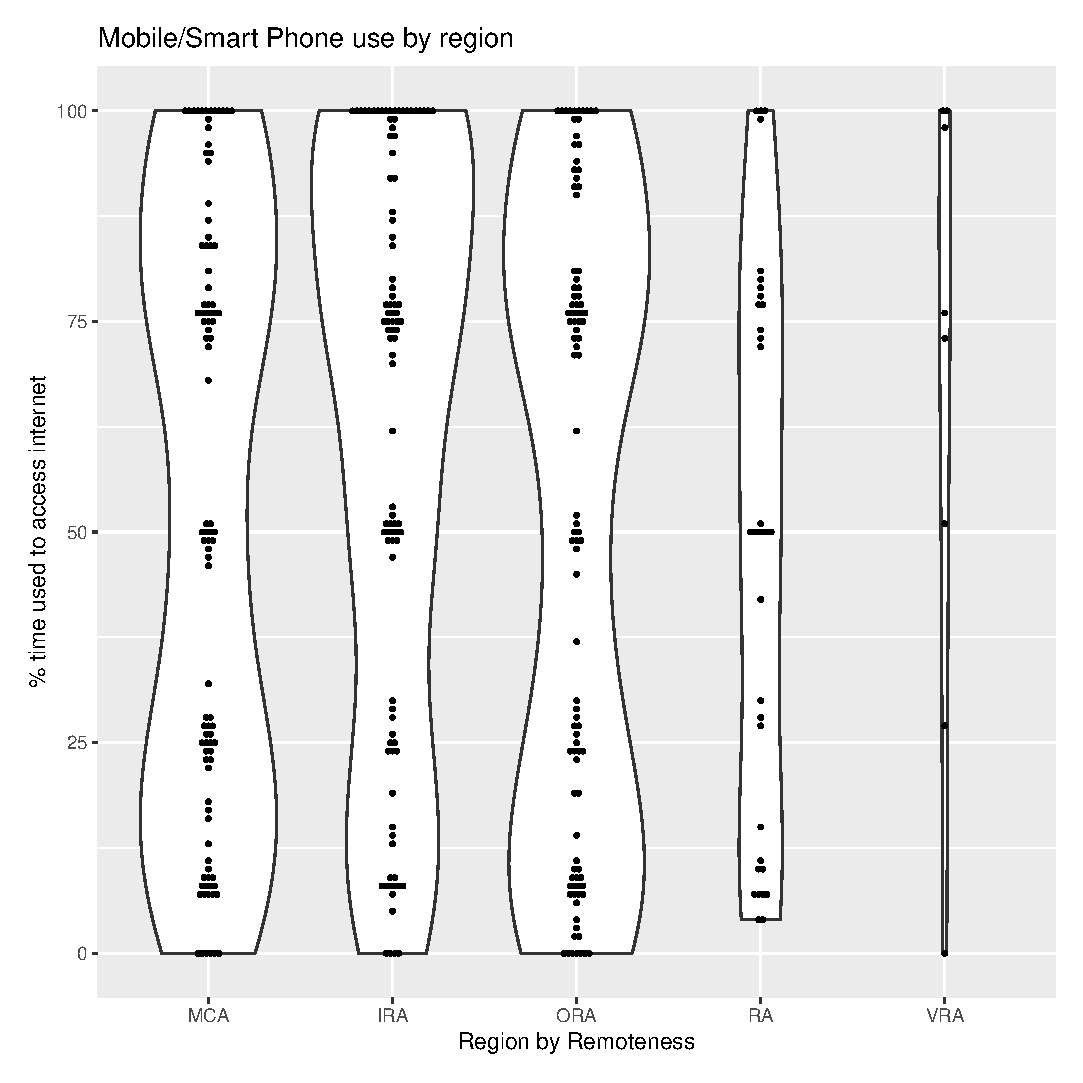
\includegraphics[scale=0.5]{figures/VChart01-MobileByRegion.eps} 
\caption{Mobile Use by Region}
\label{fig:VC01MobileRegions}
\end{figure}

This question was asked to determine whether mobile devices were the main interface between the respondents and the internet. There is a relatively uniform distribution of respondents using a mobile device to access the internet from not at all to only using mobile devices to access the internet. This uniformly tapers in Major Cities and in both Inner and Outer Regional Areas around the 50\% mark such that  the majority have a preference for either using a mobile device most of the time or not using a mobile device. This would indicate that non-mobile device access is available in all regions and that, unlike developing nations, mobile is not the preferred access technology for the internet in the areas of Australia that were surveyed.


\begin{figure}
\centering
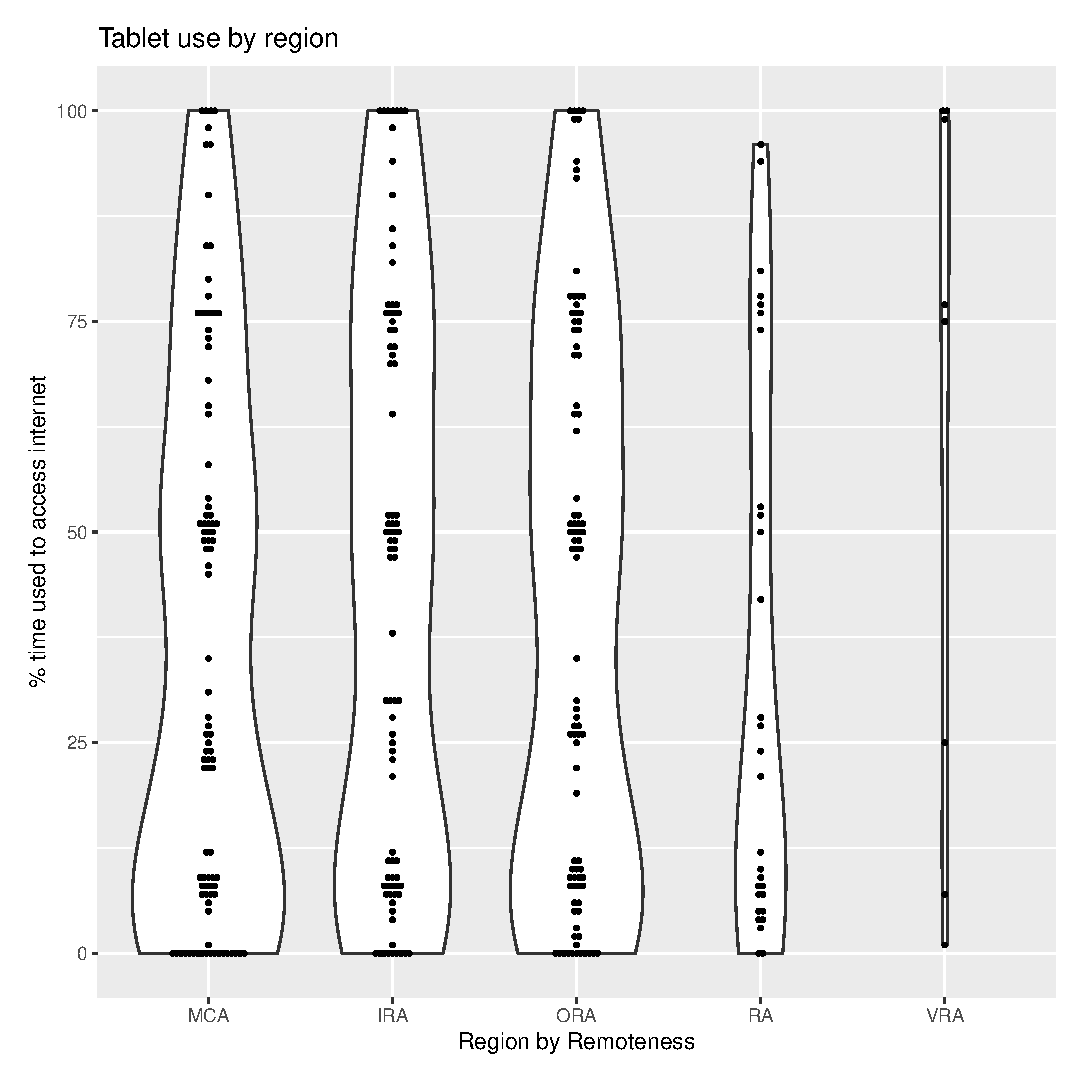
\includegraphics[scale=0.5]{figures/VChart02-TabletByRegion.eps}
\caption{Tablet Use by Region} \label{fig:VC02TabletRegions}
\end{figure}
Tablet users did show a marked preference for using their tablet devices only occasionally to access the internet with fewer respondents preferring it for 100\% of their internet accesses. Tablets are employed in all regions including Remote Areas and are seen as an occasional use technology in every region except Very Remote Areas of Australia. 
When I started this investigation in 2010 I hypothesised that cheap tablets or OneLaptopPerChild (OLPC) machines might be a way for people of limited means to gain access to computing hardware. In 2010, the idea that a laptop or any computer that could do meaningful work would be available in Australia for under \$300 was fantastic but this price was expected to be reached within ten years for quite capable hardware. Now it is possible to purchase wireless tablet hardware for under \$70\cite{RefWorks:369} that runs the latest version of Android on a four core processor which is adequate for most internet browsing. 
Even as hardware is becoming cheaper and more capable, tablet use worldwide is tapering off with Apple tablets showing stagnant growth and the market for other tablets collapsing worldwide. \cite{RefWorks:425}% need to get something from ASYMCO when they are back up.
This may be because tablets have a longer replacement cycle than mobile phones or that everyone who needs one has one that is `good enough'. As they appear from this survey and others to be occasional use devices rather than daily use devices, they can be expected to be replaced but only when they either wear out or if there is a very large shift in performance that would require much better hardware in the future over simple web browsing.

\begin{figure}
\centering
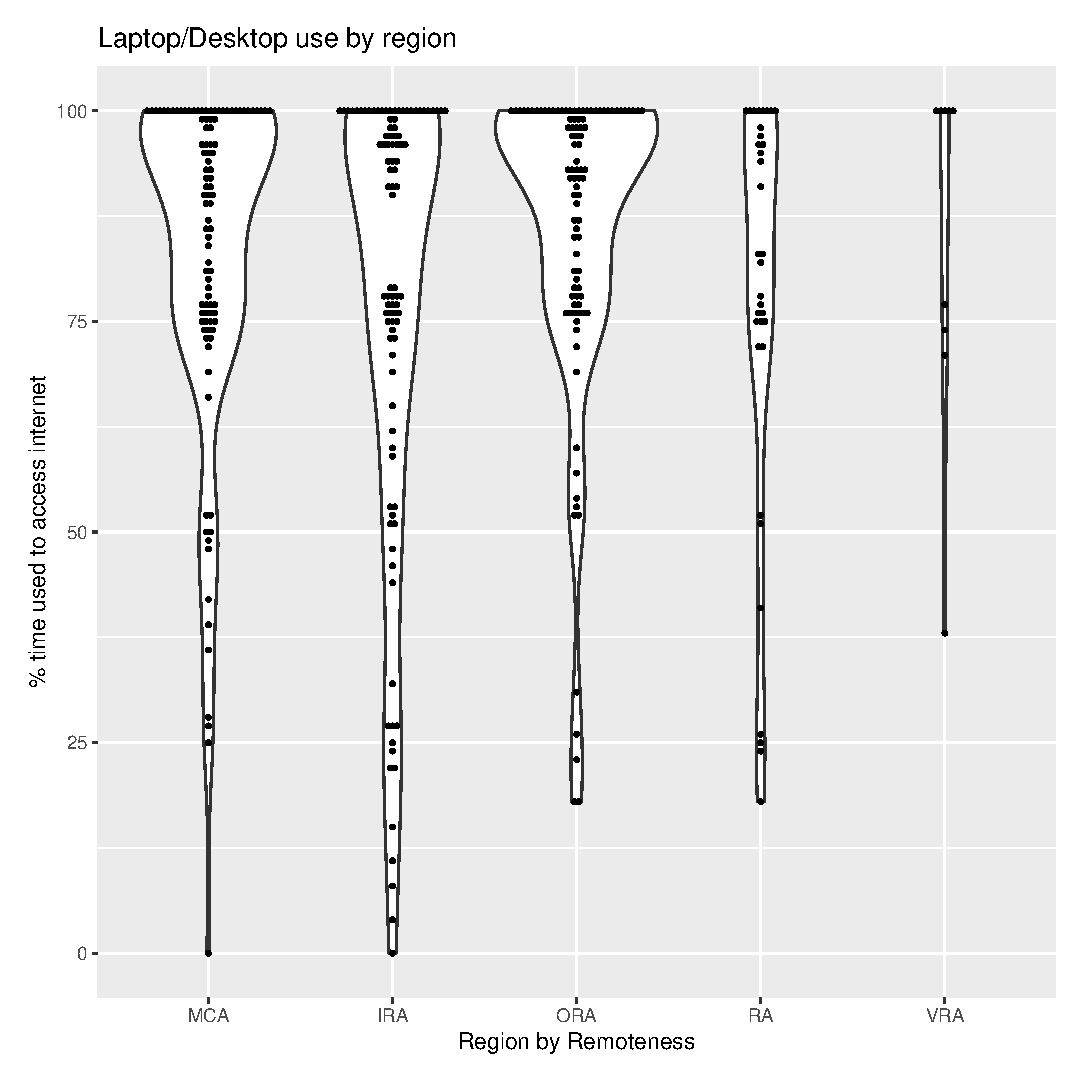
\includegraphics[scale=0.5]{figures/VChart03-LaptopDesktopByRegion.eps}
\caption{PC/Laptop/Desktop Use by Region} \label{fig:VC03LaptopDesktopRegions}
\end{figure}
Most respondents in this survey chose a desktop or laptop machine as their daily use way of accessing the internet with the majority saying that they used a desktop or laptop machine for over 75\% of the time they accessed the internet. Desktop and laptop machines have a longer replacement cycle than mobile phones and tablets, being replaced on average every five or even six years where in the past the cycle had been every three to four years.\cite{RefWorks:370}. Since few applications outside of professional graphics packages, movie rendering, high frame rate and high resolution gaming can benefit from more modern hardware, most business and home users are keeping their existing machines because they are `good enough' for the applications they purchased them to run several years ago. Incremental upgrades to storage or memory and replacing the occasional worn out component is now sufficient whereas it previous upgrade cycles it was necessary to buy a whole new PC in order to take advantage of a new operating system or program.  


Certainly the respondents to this survey have already shown themselves to be mostly Windows 10 users (Figure \ref{fig:surveyOS}) and so it is to be expected that their machines must be relatively capable. The top three resolutions reported by the survey software for these machines were 1366x768 (93 respondents), 1920x1080 (65 respondents) and 14400x900 (18 respondents). These three screen sizes make up over half the survey and relate to laptop screen resolutions or the resolution of a PC display output on a television or older monitor (see Figure \ref{fig:ScreenSize}). All support high definition (HD) movie playback indicating that, in 2016 when the survey was conducted, they were relatively well performing computers.



\begin{figure}
\centering
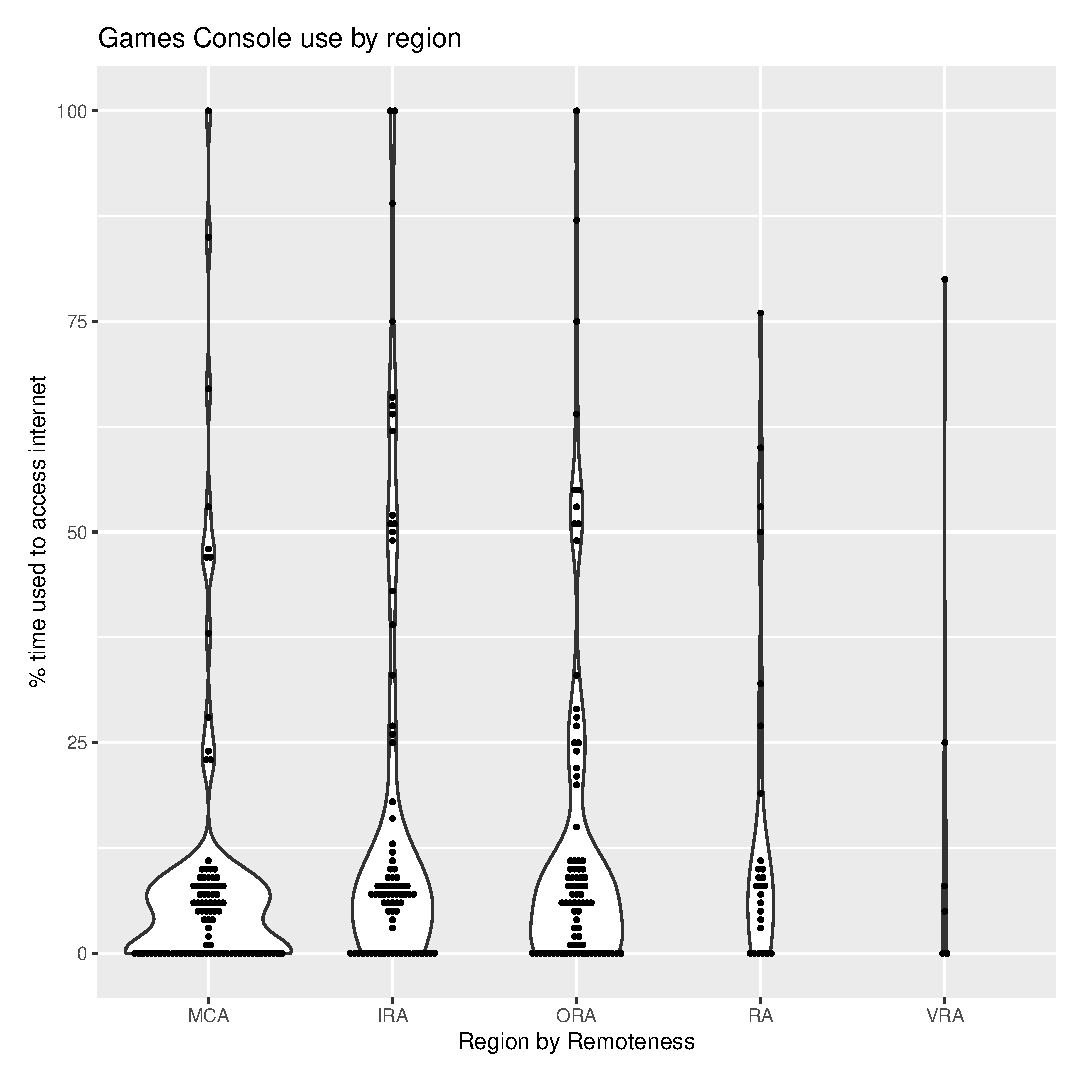
\includegraphics[scale=0.5]{figures/VChart04-GamesConsoleByRegion.eps} 
\caption{Use of Games Consoles to access the internet by Region}\label{fig:VC04GamesConsoleRegions}
\end{figure}

I included accessing the internet via games console for two reasons. Firstly, due to  research by Professor Peter Radoll in his thesis \textit{Stone Chips to Silicon Chips}\cite{RefWorks:52} which suggested that some people might only access the internet through games consoles and not use the internet for anything but multi-player online games. Secondly, because I theorised that MPOGs were becoming an important way for game players to meet and interact socially in the course of their play. 
I further theorised that, due to the large latency experienced in some internet connections in Australia, and having observed the frustrating `rubber banding' and `ganking' behaviour that results from not having a fast, low latency connection when friends and relatives played on slow ADSL connections in metropolitan Sydney, I expected that respondents in Remote and Very Remote areas would not spend a lot of time using a games console. Respondents to the survey (Figure \ref{fig:VC04GamesConsoleRegions} seem to spend only a very little time on an internet connected games console and might only use if between 10 and 20\% of the time to access the internet. This is the same for Major Cities, Inner and Outer Regional Areas and for Remote Areas. In very remote areas, games console use does not seem to be a common pastime but this may also be due to the unavailability of access to services such as Xbox Live or PlayStation Network over connections with satellite broadband and therefore high latency.

 ABS data confirms (Figure \ref{fig:absaccessmethods}) that an average of 23.1\% of homes access the internet through a games console at some time with 28.8\% of Major Cities households, using one at some time and 18.4\% of Remote and Very Remote households using one to access the internet.

\begin{figure}[ht]
\centering
\includegraphics[scale=0.75]{figures/AccessMethodByRemoteness.png}
\caption{Type of device used by households to access the internet\cite[Table 3]{RefWorks:459}\label{fig:absaccessmethods}}
\end{figure}


\begin{figure}[ht]
\centering
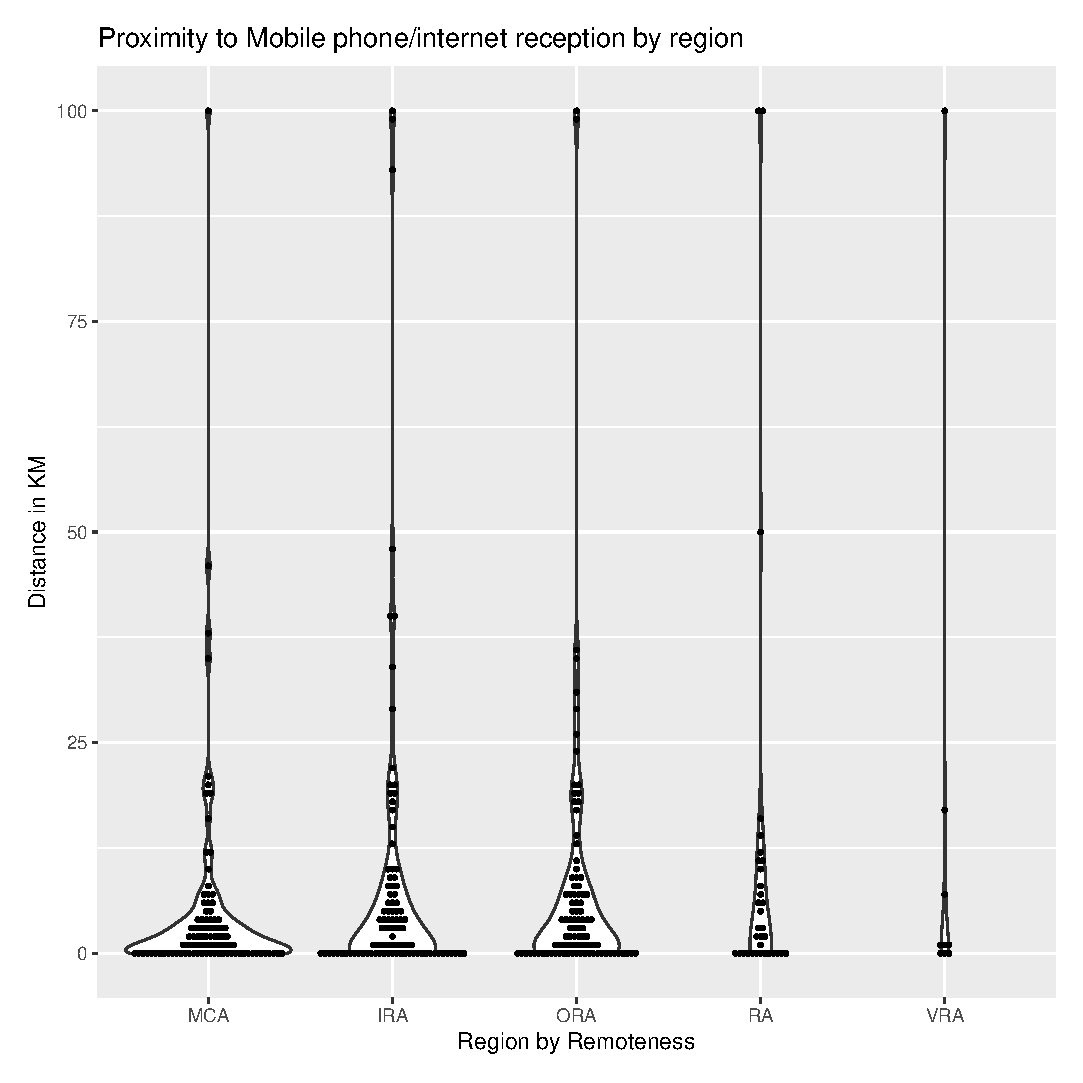
\includegraphics[scale=0.5]{figures/Vchart10-Proximity2MobileServiceArea.eps}
\caption{Distance from nearest place with Mobile phone reception by Region} \label{fig:VC010MobileAreaProxRegions}
\end{figure}


This question was designed to determine how many people in the survey had mobile phone reception and if many had to travel to obtain it. Even in Major Cities, mobile telephone reception can be unreliable but it was surprising to find that respondents in every category had many people who had to travel to obtain mobile phone or internet reception. It is a surprise to find that a large number of respondents in Major Cities still had to travel more than a kilometre and in some cases more than several kilometres to obtain mobile reception.

4G and 3G technologies have different uses. Australian telcos commonly use 3G for voice calls and 4G exclusively for data. This is changing as standards such as VoLTE (Voice over LTE) are introduced but most telco billing systems are still only able to measure and bill voice calls on 3G networks because calls made over the data network are essentially indistinguishable from other IP voice calling systems from vendors such as WhatsApp, Skype and Viber. In some countries, it is possible for LTE users to be able to use the mobile network for calls and broadband up to 75kilometres from a mobile tower but in Australia this has been limited to the same distance as 3G, 40kilometres. One of the criteria for assessing remoteness is distance from a major road and most mobile towers are positioned to either collect calls from a number of subscribers or to provide service on major roadways. Recently, the Australian Competition and Consumer Commission (ACCC) has conducted an enquiry into whether the regional mobile telephone and broadband service should be a `declared' service. This would mean that any infrastructure built in certain areas would be usable by any of the mobile service carriers that currently operate in Australia or any new entrants.

Current telco incumbents Optus and Telstra have been the major builders of mobile infrastructure outside of major cities to ensure that they can maintain a minimum standard of coverage expected by their customer base. As the inadequacy of the mobile network has become apparent over successive years it has been apparent that there is a market failure in provisioning mobile service in non-urban areas leading to mobile black spots - areas without or with unacceptable mobile service for the number of people who require it in the area. Successive governments have addressed mobile black spots with the latest round of grants going predominantly to Telstra.\cite{Battersby} Since Telstra wins most of the grants, the argument put that public money designed to address market failure is being funnelled into the incumbent building a network that only the incumbent's customers can access. Declaring the service would enable all mobile service subscribers in black spot areas to benefit from public money by allowing those customers to obtain calling and mobile broadband access and rates that are available in urban areas. 

Some services that are mostly intended for remote areas such as satellite broadband and fixed wireless are already declared services and part of the NBN. 

\begin{figure}[ht]
\centering
\wheelchart{4480/mqDarkRed/{Outer Regional},  3763/mqGreyRed/{Inner Regional}, 1171/mqRed/{Remote Australia}, 1123/mqPlum/{Very Remote Australia}, 264/mqLightPlum/{Major Cities}}
\caption{Black Spot Locations by Regional Area\cite{RefWorks:404}}
\label{fig:BlackSpotsbyRegion}
\end{figure}


\begin{figure}[ht]
\centering
\includegraphics[scale=0.3]{figures/1510coverage729px.png}
\caption{Size of largest Australian Communications carriers compared to the area their networks address\cite{Battersby}}
\label{fig:NetworkSizeVLandmass}
\end{figure}


\section{Satellite Communications}
\subsection{Aussat}
Commissioned by the Overseas Telecommunications Commission, a government body separate from the local communications authority, Telecom, in 1981, AUSSAT was responsible for the launch, operation and maintenance of a constellation of three satellites


\begin{figure}[ht]
	\subfloat[Aussat - NASA]{
	\includegraphics[scale=0.6]{figures/484x477-STS-51-I_AUSSAT_1_deployment.jpg}
		}\hfill
	\subfloat[Aussat Spot Beams]{
	\includegraphics[scale=0.4]{figures/AussatFootprint.png}
		}
	\caption{The Aussat Satellite System }
\end{figure}




As Peter White says in his article in \textit{The Australian}, the Aussat system was hugely expensive.

\begin{quotation}
\ldots the government inquiry proposed a more costly, cutting-edge system that, among other things, could broadcast to homes using low-cost ground stations. People in remote and rural Australia would be able to receive TV, radio and reliable telephone service for the first time. TV and radio broadcasters would be able to share programming in real time and businesses would be able to create data links between distant premises. A great deal was made of the benefits for the School of the Air in the outback and the potential for tele-medicine.

[However\ldots]

Aussat came to a sticky end. Telecom Australia created a terrestrial telephone system for remote users independent of Aussat. 
The \$1,000 television and radio ground stations promised by the government cost much more than predicted. (The government scrambled to reduce their price by removing taxes and duties but the ground stations were still too expensive for many remote and rural residents.) The School of the Air and its clients struggled to purchase the expensive equipment needed for two-way communications and extended tele-medicine usage never really took off. Predicted revenues were not achieved and Aussat generated large losses\cite{RefWorks:60}.
\end{quotation}

The true cost of this failure became apparent when fibre optic cables began to overtake satellite technology. The ramp-up required for the satellite, and the non-availability of suitable launch vehicles, the relatively small size of the satellite that was necessitated by its target launch vehicle (the NASA/Boeing Space Shuttle) and the relatively uncertain and inherently risky nature of satellite launches at the time meant that the system was over budget and old fashioned by the time it began to compete with fibre optic cables that had been laid between capital cities in the meantime.
\begin{quotation}
The Australian television industry utilizes satellite technology for two purposes, program distribution and remote broadcasting. In terms of distribution, satellite technology has dramatically escalated costs in an industry squeezed by high gearing ratios and stagnant revenue levels. The industry's plight was graphically illustrated by Northern Star writing off \$514m in the sale of the Ten Network in September 1989. The benefits of networking which the satellite system was to usher in and for which long held principles of diverse media ownership were sacrificed, have simply not materialized.

The commercial broadcaster's technical costs, as reported to the ABT, have dramatically risen since the advent of Aussat. In the year following the shift to satellite the industry's capital city stations reported a 222\% increasing combined technical costs from \$12m to \$26.7m In 1987/88 technical costs rose to \$33.3m. This contrasted to the years leading up to 1985 when real costs had been falling.

\ldots

Cost increases have led the networks to closely examine the need for satellite distribution. For program distribution Telecom's inter-city fibre network represents a technically superior and more cost efficient option for Aussat's existing customers. Broadcasters are now in the position of being able to play off Aussat and Telecom against one another\cite[p333]{RefWorks:334}.
\end{quotation}

This scheme finally delivered around 60 small low powered television/radio stations that were capable of taking broadcast television and radio via satellite dish and retransmitting it. In the event, AUSSAT was sold to Optus (ibid) as a requirement of its taking a telecommunications license as Australia's second Communications Service Provider (CSP) and much of the benefit of remote and regional television reticulation was realised by a new organisation called the \emph{Broadcasting for Remote Aboriginal Communities Scheme} (BRACS). Elizabeth Jacka's article on the subject, \emph{The Australian Media Landscape: Recent Changes} \cite{RefWorks:59} is a good history of the implementation of AUSSAT. 


\subsection{NBN Sky Muster satellite}
Sky Muster is the trademark name given by the NBN to its high capacity satellites that are designed to distribute next generation broadband services to remote and inaccessible regions of Australia that cannot be reached by cabled or fixed wireless connections. It addresses all those areas of Australia and it's territories (it has spot beams that can reach the Australian Antarctic territory of Macquarie Island as well as territorial islands such as Cocos Islands, Christmas Island, Norfolk Island and Lord Howe Island. 
The satellite uses 101 `spot beams' or antenna's focussed on either a wide or narrow footprint of land to send and receive packets of data. It is a very large satellite with a mass of 6,400kg that is just under ten times heavier than the original Aussat mass of 654kg.
\begin{figure}[ht]
\subfloat[Sky Muster II at Space Systems Loral's assembly facility in Palo Alto, CA \cite{RefWorks:339}]{
\includegraphics[scale=0.3]{figures/Skymuster.png}
}
\hfill
\subfloat[Sky Muster Spot Beams \cite{RefWorks:340}]{
	\includegraphics[scale=0.45]{figures/SkymusterSpotbeams.png}
}
\caption{The Sky Muster Satellite}
\end{figure}


\subsection{NBN Fixed Wireless}
While mobile devices in moving vehicles need to employ special protocols to allow them to communicate with a base station while moving at up to 500kmph, most mobile devices in remote areas of Australia are not moving as fast as a TGV passenger train or light aircraft. The NBN has taken the decision to use a form of LTE called fixed wireless where the receiving point is attached to a stationary object such as a house or farm outbuilding and a WiFi hotspot or cabled connections taken from that to serve residents. This has the property of doubling the distance from the access point to the mobile phone tower and does so at 4G LTE speeds rather than having to use satellite technologies. As well as having a higher speed on average, than satellite, it is possible to offer download quotas that are similar to wired connections and so avoid the broadband caps that are in use on commercial 4G services from mobile phone carriers. The NBN, however, has decided to limit fixed wireless to a distance of 14km and in some cases the distance is as low as 6km.\cite{RefWorks:331}

\begin{figure}[ht]
\centering
\includegraphics[scale=0.5]{figures/satellite-beamsFW.png}
\caption{Satellite Congestion survey results - Fixed Wireless Review}
\label{fig:satbeams}
\end{figure}

Fixed wireless is preferable to satellite in all cases. It is more immune to rain fade, it has minimal latency because the signal need only propagate from the mobile terminal (the smart-phone, tablet or computer) to the mobile base station and will then be on fibre optic to the nearest Point of Interconnect (POI). NBN is filling in many areas that would have otherwise merited service from the Sky~Muster satellite with fixed wireless to remove the load from the satellite in areas of likely congestion. As shown in Figure~\ref{fig:satbeams}, areas where spot-beams are congested are targeted for Fixed Wireless infill to relieve the pressure on beams in that area and allow satellite subscribers to get acceptable service. The more users in each cell the lower the bandwidth available. 

The Sky Muster satellite system aggregates requests for internet packets from terminals inside each spot beam footprint and passes those to an earth station to be served over the internet. The Sky Muster system has nine earth stations in areas unlikely to be affected by rain fade to pass the requests to  the internet through a `meeting place' in Sydney. This means that if a request is handed over to an earth station in Western Australia, there will be an additional latency introduced while the signal travels to Sydney from Western~Australia and back again to be sent back to the satellite and then back down to the originating spot-beam. The spot-beams are allocated earth stations based on the capacity of the spot-beam and terminals can be reallocated every ten minutes depending on the load on that particular spot. This may mean that a terminal in Western~Australia, Port~Headland for example, is allocated an earth station in Queensland (Roma) which would have a lower round trip latency than another location that was allocated a West~Australian ground station such as the ACT which is currently allocated a Western Australian Earth station due to capacity constraints on the New~South~Wales earth stations.\cite{RefWorks:340}

The current Sky Muster system has had many teething problems with poor download speeds, buggy modems and a lack of plans that are equivalent to cabled connections or even to mobile broadband plans. As the service is being tuned and load is being diverted to fixed wireless, some of these issues are being resolved but geostationary satellite communications will never be as fast as terrestrial internet due to the propagation delay.

Like other countries using similar technology, Australian consumers will have to wait for other solutions in the future to equalise the quality of service between very remote and remote areas and urban centres.


\section{Future Technologies}
Other technologies are being developed that will provide internet service to remote and very remote areas, in some cases over the entire Earth. They are designed to remove the problem of propagation delay inherent in the round trip time taken from terminal to geostationary satellite to earth-station and back again. Geostationary satellites are typically positioned around 36,000kms above the Earth's surface. At this distance they have to faster than 11,000kmph to have an orbital period equivalent to a day and appear to hover over the same location on earth. The time taken for a signal to travel from the ground to the satellite is over twice that of the time taken to travel from one side of the Earth to the other at 270 milliseconds one way or 540 milliseconds for a round trip.

If satellite communications are to offer similar latencies and bitrates to cable based or even mobile broadband solutions then they have to have a way to remove the round trip latency issue. Low Earth orbit satellites have been used in the past and LEO solutions are proposed for the future as well as other technologies that will deliver speeds equivalent to current ground based access technologies.

\begin{figure}[ht]
\centering
\includegraphics[scale=0.75]{figures/NextgenInternet.png}
\caption{Future internet delivery technologies for remote areas that \cite{RefWorks:354}}
\label{fig:FutureInternet}
\end{figure}


\subsection{Iridium constellations}
The Iridium satellite system consists of a constellation of satellites moving in low earth orbit of 780km above the Earth and at this distance the round trip time from satellite to earth station is between 4.3 and 7.8 milliseconds or 15.6 milliseconds for a round trip and the satellite's speed must be over 27,000kmph to complete an earth orbit every 100 minutes or it will fall out of orbit. Iridium satellites are capable of directing traffic between each other and can pass communications packets between satellites if they are orbiting in the same direction. This would be useful if, for example, a person on a ship was communicating with their head office and with one Iridium satellite being able to see both the ship and another Iridium satellite that could see the head office. This would avoid two legs of a trip and shave vital milliseconds off latency. Iridium originally intended that there would be 77 satellites in the constellation (77 is the number of Iridium in the periodic table) but it was found that the constellation could practically cover the inhabited surface of the Earth with only 72 satellites, 66 in operation and six as in-orbit spares\cite{RefWorks:342}.

\begin{figure}[ht]
\centering
\includegraphics[scale=0.75]{figures/iridium_global_network.png}
\caption{Iridium NEXT --- Low Earth Orbit Constellation\cite{RefWorks:343}}
\label{fig:iridium}
\end{figure}

The existing constellation has a very low bitrate, communicating with earth terminals at 10kilobits per second, around the speed of dial up modem that was common in the decade it was launched. The current system supports under 600,000 users which is around the same number of users that Sky~Muster supports at between 12Mbps to 25Mbps. Its main customers are the military and government and research organisations that find the ability to connect instruments and communicate from anywhere on the planet necessary to their missions.

While it is technically impressive, the bandwidth of the Iridium constellation is not acceptable for contemporary internet communications at scale in the remote and very remote areas of Australia. It is sufficient for emergency phone calls or very low bandwidth telemetry but it's latency, bandwidth and capacity constraints make it unsuitable for the scale of the population in remote areas of Australia. Iridium is using SpaceX launch vehicles to replace every one of their 72 satellites with upgraded `Iridium~NEXT' satellites that can communicate at between 1Mbps to 8Mbps with a latency of 15.6 milliseconds round trip. Every launch replaces 10 satellites with the next generation model and so far there have been two launches. This project is due to be realised in 2018 when it will continue to largely serve its existing customer base\cite{RefWorks:343}. 

There are systems from other vendors being created and launched now in anticipation of providing the same seamless global service but at latency and bandwidth levels similar to current ADSL cabled connections. Other companies, ViaSat and Globalstar can offer similar services to Iridium~NEXT but if any system is to hope to provide world wide coverage to serve all the very remote and remote regions of the Earth, a large scale solution is called for. Some prospective solutions come from SpaceX, the company currently launching the Iridium replacement satellites, Google with their Loon project and Facebook who are working on a drone based system to provide seamless global internet connectivity.  SpaceX, Google and Facebook all have the goal to connect the last two billion people who are currently not served by the internet. The emerging markets of Africa and South~America provide uncontested areas where a free internet service, provide by serving customers to advertisers in the case of Facebook and Google. SpaceX expects to make more profits from its satellite constellation by selling the high quality, high speed internet service than it does from its space launches by 2025. 

 
\subsubsection{Google Loon}
Google is developing a balloon based system of internet relays where a network of balloons floating on well mapped global air currents move through the stratosphere like boats sailing in a river that moves at roughly the same speed worldwide. The balloons can control their altitude by means of a ballast balloon of air inside the main helium balloon that keeps the Loon aloft. When taking on air from the outside, the Loon descends and when it discards it, it rises. Since the air currents move in different directions at different altitudes, it is possible for the flock of balloons to navigate their way over the entire surface of the planet

Google believes it's business may be bigger than it's current YouTube business once Loon is running worldwide. They forecast a market of 4.5 billion internet customers who are currently non-consumers due to there being no service in their area. Google Loon will use the incumbent carrier's infrastructure to connect to the communications network in the country it is flying over to provide mobile cell towers in areas where the incumbent would find it prohibitively expensive to provide service.

Since each balloon only lasts around six months before needing to be replaced, the Loon fleet is capable of undergoing a continual technology refresh and take advantage of higher capacity LTE systems that use less power and better battery and solar panel systems.
\begin{figure}[ht]
\centering
\includegraphics[scale=0.25]{figures/merlin.png}
\caption{A Google Loon balloon showing the internal `balloonlet' that manages altitude to aid navigation\cite{RefWorks:360}}
\label{fig:loon}
\end{figure}
\begin{quotation}
The team recently crossed another milestone with its first successful connection test across multiple continents. Balloons launched in New Zealand flew over 9,000 kilometers (about 5,600 miles) to Latin America and delivered an internet connection, then flew back around the globe for another successful connection test in Australia, navigating the balloons within 500 meters of their target locations at opposite ends of the world.

Google wants to work with, not against the incumbent Telcos and connect to the network of the country the balloon is flying over to provide service. 

Loon has now conducted tests with Vodafone in New Zealand, Telstra in Australia, and Telefonica in Latin America, and it says it’s working on commercial deals with several new network operators around the globe. These companies already own the spectrum and have the infrastructure in place to market, sell, and bill customers for service. Google gets permission to use the spectrum and provides the cell towers in the sky, sharing the revenue for each new customer with the telco.
\end{quotation}

Google Loon has shown it is capable of serving areas where natural disasters have disabled the existing rural communications network, most recently in Peru and so it may be used in the same way as Telcos in Australia use mobile base stations known as Cells on Wheels (COWs) to provide service to areas that are involved in a natural disaster such as bushfire or flood or to provide short term augmentation when a large event such as the Birdsville Races increases a regional town's population beyond the capacity of the local mobile broadband service\cite{RefWorks:348}. It is particularly important to Australia as the current test system uses the `roaring forties' winds that are among the most reliable continuous wind system on the planet and pass over Australia's Bass Strait  near Melbourne and Tasmania and over Wellington, New~Zealand. Users will be able to use their moblie phones or LTE enabled tablets to communicate with the network and each Loon has a coverage area of 5000 square kilometres\cite{RefWorks:343}.  


\subsubsection{Facebook drones}
Facebook has a mission to connect people who cannot currently access the internet to it. It is provisioning a free service through it's `walled garden', internet.org, which provides mobile service in 42 nations access to community services such as wikipedia, local health services information and, of course, a version of facebook that is designed to load quickly on low bandwidth mobile devices such as 2G mobile phones.  Facebook has so far achieved this by cooperating with local Telcos in the same way Google is working with many local telcos to connect it's users to Loon services. This has been problematic for Facebook in two key markets, India and Egypt, where their license to provide a service has been cancelled. While no official reason has been given, in Egypt, facebook was a key element that allowed the orchestration and coordination of the movement known as the `Arab Spring' in 2011 that toppled the Egyptian president, Hosni Mubarak and there has been concern that this has made the current authorities wary of any Facebook services they don't control\cite{RefWorks:356}.


\begin{figure}[ht]
\centering
\includegraphics[scale=0.5]{figures/AquilaStats.png}
\caption{internet.org and the Aquila drone\cite{RefWorks:358}}
\label{fig:Aquila}
\end{figure}

Facebook has determined to move away from total reliance on local mobile service operators and has a future strategy of deploying High Altitude Long Endurance (HALE) drones. Facebook were attempting to design their own aircraft, known as `Aquila' for this purpose but aircraft manufacturer Airbus already has a commercial model, the Zephyr, that is currently employed for similar, military, missions where communications and surveillance are required\cite{RefWorks:358}. The drones were to  be solar powered and be stationed in the same region of airspace above a service location for weeks or months at a time. At an altitude of between 60,000 and 90,000 feet (18 to 27 kilometres), the latency for an internet drone will be under 1 millisecond for a round trip from the ground to the drone and back again. Drones can communicate both with ground stations for uplink and with other drones via laser to relay packets around the network to enable them to reach far from the ground station without additional uplink towers being installed at ground level and allowing the network to be reconfigured on command rather than having to orchestrate a movement based on wind currents as with Google Loon. Like Google Loon, drones will have to return to earth after their extended mission aloft which would allow the upgrading of on-board equipment whereas a LEO or geostationary satellite solution is not easily upgradable for new communications technologies.

Like Loon, a drone delivery  model has shown its service model to be vulnerable to termination by the sovereign territories that it overflies. Using drones in concert with a walled garden internet would limit interaction with other parties on what is supposed to be an open network. In this network model, communications would need to be mediated by a third party both for the physical layer of the network itself and for the content on the information conveyed to the users. While the drones fly higher than commercial aircraft, they are still subject to the airspace restrictions and telecommunications regulations of the countries they operate in. Facebook had intended to deploy a communications satellite, the AMOS-6, to test using satellites to provide internet access over sub-Saharan Africa. Unfortunately this satellite was destroyed in a refuelling incident before launch\cite{RefWorks:460} and Facebook has temporarily shelved the idea. 


\subsection{SpaceX satellite constellation}
SpaceX has proposed a system of 4,425 satellites that will be launched between 2019 and 2024. To put this into perspective, ``There were an estimated 1,459 operating satellites orbiting Earth at the end of 2016, and the 4,425 satellites in SpaceX's planned initial launch would be three times that many\cite{RefWorks:343}.'' SpaceX proposes that these satellites will orbit in 80 orbital planes at altitudes between 1,110km to 1,325km. They anticipate a latency of no more than 25milliseconds round trip time which is equivalent to existing ADSL solutions but slower than some fibre, vDSL and HFC technologies currently deployed in Australia. SpaceX have an upgrade path that involves deploying an additional 7,500 \gls{vleo} satellites to ensure low latency and increase capacity.
 
The SpaceX \gls{vleo} solution is both Ka and Ku band solution which will give it some protection against rain fade and allow increased service availability over Ku based solutions such as Sky Muster but SpaceX's solution is not designed solely for Australian conditions or even for remote and very remote conditions, it is designed to be able to provide service in any uncontested market for internet services worldwide. 
\begin{quotation}
A January [2017] Wall Street Journal report examining leaked SpaceX documents revealed that the company expects its internet business to earn more than its rocket launches by 2020. It projects that the business will have 40 million subscribers and earn \$30 billion in revenue by 2025. In total, SpaceX pulled in \$945 million in revenue in 2015\cite{RefWorks:347}.
\end{quotation}

The question will not be whether SpaceX can make enough profit to make it worth their while investing in infrastructure in Australia as their constellation of satellites will fly continuously over the entire mass of the Country and its territories on their way to even more populous and profitable customers in developing economies such as Africa, South America, Russia and all the countries between it and China and India. It will serve areas that cannot be reached by current technology in Europe, the United States, planes in flight and ships at sea with ubiquitous internet service that is the equivalent of current DSL quality. Unlike the Google Loon or Facebook Aquila it cannot be casually shot down and the terminals are small enough that their operation will be more difficult to regulate than systems that might require large satellite dishes to concentrate a signal on a geostationary satellite. Unlike mobile phone towers which can be turned off by hostile forces in war zones or contested political areas, the SpaceX satellites pass over their service area within a few minutes to be replaced by another solar powered, communications beacon. For those areas that are not well served by the NBN Sky~Muster satellite it will provide an alternative. 

While the Australian government may move to make the provision of internet services by any of these three providers illegal it is difficult to see what the motivation for reducing competition would be aside from protecting vested interests and instituting government censorship of the internet. It is clear that there are several alternative technologies that will be available as alternatives to the NBN Sky~Muster satellite solution for remote and very remote internet access in the next few years.

\section{Conclusions}
Access to the physical internet will continue to improve in Australia. Speeds and download quotas will improve but not as fast as the rest of the world. Services are migrating to the internet and access to the internet is already essential to have the same standard of living and efficient and economical access to government services, health, education and financial services that are typical for urban Australians. Private networks being built to take advantage of 4G and 5G technologies by both the government led NBN and private telecommunications companies may be eclipsed by over the top services from internet companies such as Facebook and Google or by satellite communications systems launched by Space X and others that will provide satellite and other technologies faster and more ubiquitously than the NBN's fixed wireless and satellite options. Australians are now served by a satellite system accessible both on the ground, in moving vehicles and even from planes in flight over the continent. For the first time all Australians can access the internet and the required hardware is available and inexpensive. The remaining barriers to access of affordability, propensity to use and appropriate services still need to be solved for all Australians to gain full advantage from the ICT.
